\documentclass[5pt]{article}
%\usepackage{fontspec}
%\setsansfont{Roboto Condensed}
\usepackage{multicol}
\usepackage{calc}
\usepackage{ifthen}
\usepackage[landscape]{geometry}
\usepackage{amsmath,amsthm,amsfonts,amssymb}
\usepackage{color,graphicx,overpic}
\usepackage{hyperref}
\usepackage{gensymb}
\usepackage[normalem]{ulem}
\usepackage{dashundergaps}
\usepackage{makecell}
\usepackage{tabu}

\usepackage[sfdefault, condensed]{roboto}
\geometry{top=0.5cm,left=0.5cm,right=0.5cm,bottom=0.5cm}
%I would do the following,
%1. Review the lectures for the theoretical parts (this is the multiple-choice questions)
%2. How the open loop gain and the closed loop gain are linked to each other and which open loop gain you need for a certain accuracy, how to get the gain in dB
%3. Review how to get the transfer functions of amplifiers (inverting, non-inverting amplifiers, superposition principle to be able to get the CMRR, the differential mode gain of amplifiers).  Remember also virtual ground property of amplifiers to simplify much analysis
%4.Sensors types are important (especially resistive, capacitive, and temperature sensors)
%5.DAC types and how to get INL and DNL
%6.Taylor series to approximate functions as I told you in the exercise session

% This sets page margins to .5 inch if using letter paper, and to 1cm
% if using A4 paper. (This probably isn't strictly necessary.)
% If using another size paper, use default 1cm margins.
%\ifthenelse{\lengthtest { \paperwidth = 11in}}
%    { \geometry{top=.5in,left=.5in,right=.5in,bottom=.5in} }
%    {\ifthenelse{ \lengthtest{ \paperwidth = 297mm}}
%        {\geometry{top=1cm,left=1cm,right=1cm,bottom=1cm} }
%        {\geometry{top=1cm,left=1cm,right=1cm,bottom=1cm} } 
%    }

% Turn off header and footer
\pagestyle{empty}

% Redefine section commands to use less space
\makeatletter
\renewcommand{\section}{\@startsection{section}{1}{0mm}%
                                {-1ex plus -.5ex minus -.2ex}%
                                {0.5ex plus .2ex}%x
                                {\normalfont\large\bfseries}}
\renewcommand{\subsection}{\@startsection{subsection}{2}{0mm}%
                                {-1explus -.5ex minus -.2ex}%
                                {0.5ex plus .2ex}%
                                {\normalfont\normalsize\bfseries}}
\renewcommand{\subsubsection}{\@startsection{subsubsection}{3}{0mm}%
                                {-1ex plus -.5ex minus -.2ex}%
                                {1ex plus .2ex}%
                                {\normalfont\small\bfseries}}
\makeatother

% Define BibTeX command
\def\BibTeX{{\rm B\kern-.05em{\sc i\kern-.025em b}\kern-.08em
    T\kern-.1667em\lower.7ex\hbox{E}\kern-.125emX}}

% Don't print section numbers
\setcounter{secnumdepth}{0}


\setlength{\parindent}{0pt}
\setlength{\parskip}{0pt plus 0.5ex}

%My Environments
\newtheorem{example}[section]{Example}
% -----------------------------------------------------------------------

\begin{document}
\raggedcolumns
\raggedright
\footnotesize
\begin{multicols*}{2}


% multicol parameters
% These lengths are set only within the two main columns
%\setlength{\columnseprule}{0.25pt}
\setlength{\premulticols}{1pt}
\setlength{\postmulticols}{1pt}
\setlength{\multicolsep}{1pt}
\setlength{\columnsep}{2pt}

\begin{center}
     \Large{\underline{TMS II}} \\
 
\end{center}


% Summary starts here
% --------------------------------------------------------------------------------------
\subsection{Begriffsdefinitionen}
\subsubsection{Konfigurationsmanagement}
KM stellt sicher, dass Produkte eindeutig identifizierbar sind, Zusammenhänge und Unterschiede von
verschiedenen Versionen einer Konfiguration erkennbar bleiben und Produktänderungen nur kontrolliert durchgeführt werden können.
Arten der Durchführung:
- Automatisch (z.B. Git)\\
- Manuell\\
- Semi-automatisch (z.B. unterstützende Plugins)\\
\textbf{Build-Management}\\
Unter Build-Management wird diejenige Funktion verstanden, die alle Bauteile einer Konfiguration
erzeugt, die nicht direkt vom Benutzer erstellt oder durch das System vorgegeben wurden. Zentrale Fragen: Wie ist die Software zusammengestellt? Welche Abhängigkeiten müssen berücksichtigt werden? Beispiele für klassische Abhängigkeiten:
o Entwicklungsumgebung: Editor, Generatoren, Compiler, Linker, …\\
o Basissoftware: LAN, ...\\
o Betriebssystem\\
o Hardware\\
\textbf{Change-Management}\\
Im Änderungswesen muss definiert werden, wie Änderungswünsche (Change Requests) erfasst
werden, wie und durch wen diese bewertet werden und wie die Durchführung von Änderungen
zu erfolgen hat.\\
- Versions-Management (Wer hat wann was geändert?)
Versionsmanagement befasst sich (in erster Linie mit der Verwaltung der zeitlich aufeinander folgenden Revisionen eines Dokuments.)
\textbf{Release-Management}\\
Ein Release ist eine an Kunden ausgelieferte Konfiguration eines (Software-)Systems, bestehend
aus ausführbaren Programmen, Bibliotheken, Dokumentation, Quelltexten, Installationsskripten
und so weiter. Das Release-Managementdokumentiert ausgelieferte Konfigurationen und stellt
deren Rekonstruierbarkeit sicher.
Geplant
\subsubsection{Produktzustände}
\textbf{In Bearbeitung}\\
Das Produkt wird bearbeitet. Es befindet sich entweder im privaten Entwicklungsbereich des
Entwicklers oder unter Kontrolle des Entwicklers innerhalb der Produktbibliothek.\\
\textbf{Vorgelegt}\\
Das Produkt ist aus der Sicht des Erstellers fertig und wird der Konfigurationsverwaltung übergeben. Ab jetzt kann es einer Prüfung durch die Qualitätssicherung unterzogen werden. Wird das
Produkt hierbei abgelehnt, so geht es wieder in den Zustand in Bearb. zurück, andernfalls rückt
es in den Zustand akzeptiert vor. Ab dem Zustand vorgelegt an kann der Ersteller nur unter
Fortschreibung der Versionsangabe Modifikationen durchführen.\\
\textbf{Akzeptiert}\\
Das Produkt wurde durch die QS überprüft und freigegeben. Es darf nur noch innerhalb einer
neuen Version geändert werden.
\section{CTL}
\subsection{Zustandsautomat als Zustandsraum}
Zustandsraum endet mit Übergängen\\
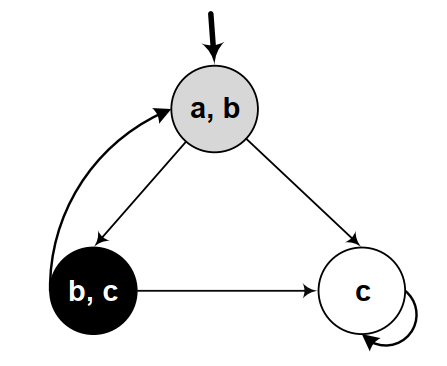
\includegraphics[width= 0.3\columnwidth]{images/bspAutomat.png}
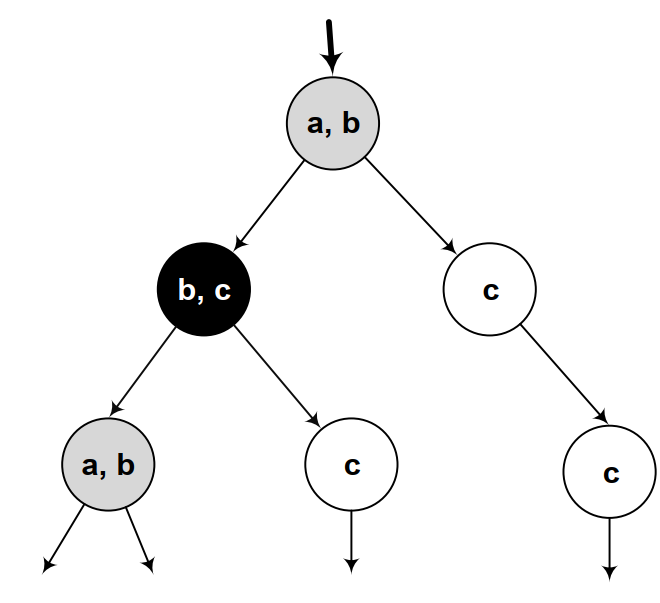
\includegraphics[width=0.3\columnwidth]{images/bspRaum.png}
\columnbreak
\subsubsection{Pfadoperatoren:}
- $A \phi$ - auf allen Pfaden folgt $\phi$ (englisch: AIl) \\ 
- E $\phi$ - auf mindestens einem Pfad folgt $\phi$ (englisch: Exists) \\ 
\subsubsection{Pfad-spezifische Operatoren:}
- $X \phi$ - unmittelbar folgt $\phi$ (englisch: neXt state) \\ 
- $F \phi$-irgendwann folgt $\phi$ (englisch: some Future state oder Finally) \\ 
- $G \phi$ - auf dem folgenden Pfad folgt in jedem Zustand $\phi$ (englisch: Globally) \\ 
- $\phi U \psi-\phi$ folgt bis zum Erreichen des Zustands $\psi$ (englisch: Until) \\ 
- $\phi W \psi-\phi$ folgt immer oder bis zum Erreichen des Zustands $\psi$ (englisch: Weak Until) \\ 
- $E X \phi$ - in (mind.) einem nächsten Zustand gilt $\phi$ \\ 
- $E F \phi$ - in (mind.) einem der folgenden Zustände gilt $\phi$ (AG EF Terminal) stellt Terminal sicher\\ 
- EG $\phi$ - es gibt (mind.) einen Pfad, so dass $\phi$ entlang des ganzen Pfades gilt \\ 
- $E[\phi U \psi]$ - es gibt einen Pfad, für den gilt: bis zum ersten Auftreten von $\psi$ gilt $\phi$ \\ 
- $A X \phi$ - in jedem unmittelbar nächsten Zustand gilt $\phi$ \\ 
- AF $\phi$ - man erreicht immer einen Zustand, in dem $\phi$ gilt \\ 
- $A G \phi$ - auf allen Pfaden gilt in jedem Zustand $\phi$ \\ 
- $A[\phi U \psi]$ - es gilt immer $\phi$ bis zum ersten Auftreten von $\psi$ \\ 
\subsubsection{Semantik}
- $T\left(s_0\right) \models \neg \phi \quad \Leftrightarrow \quad T\left(s_0\right) \not \models \phi$ \\ 
- $T\left(s_0\right) \models \phi \vee \psi \quad \Leftrightarrow \quad T\left(s_0\right) \models \phi \operatorname{oder} T\left(s_0\right) \models \psi$ \\ 
- $T\left(s_0\right) \models E X \phi \quad \Leftrightarrow \quad T\left(s_1\right) \models \phi$ \\ 
- $T\left(s_0\right) \models E G \phi \quad \Leftrightarrow \quad \forall i: T\left(s_i\right) \models \phi$ \\ 
- $T\left(s_0\right) \models \phi E U \psi \quad \Leftrightarrow \quad \exists k: T\left(s_k\right) \models \psi \wedge \forall i<k: T\left(s_i\right) \models \phi$ \\ 
\subsubsection{Transformationen} 
- $\neg A \phi \equiv E \neg \phi$ \\ 
- $\neg A F \phi \equiv E G \neg \phi$ \\ 
- $\neg E F \phi \equiv A G \neg \phi$ \\ 
- $\neg A X \phi \equiv E X \neg \phi$ \\ 
- $A G \phi \equiv \phi \wedge A X A G \phi$ \\ 
- $A G \phi \equiv \neg EF (\neg \phi)$\\
- $E G \phi \equiv \phi \wedge E X E G \phi$ \\ 
- $A F \phi \equiv \phi \vee A X A F \phi$ \\ 
- $E F \phi \equiv \phi \vee E X E F \phi$ \\ 
- $A[\phi U \psi] \equiv \psi \vee(\phi \wedge A X A[\phi U \psi])$ \\ 
- $E[\phi U \psi] \equiv \psi \vee(\phi \wedge E X E[\phi U \psi])$
\subsection{Wahrheitstabelle}
$    \begin{array}{|c c|c|c|c|}

    p & q & p \land q & p\lor q  & p \rightarrow q  \\ 
    \hline % Put a horizontal line between the table header and the rest.
    T & T & T& T& T\\
    T & F & F& T& F\\
    F & T & F& T& T\\
    F & F & F& F& T\\
    \end{array}
 $
 \columnbreak
\section{Aufwandsschätzung}
% Einheiten Leistung und arbeit durch hinzukommende hinzufügen in ml
\subsection{Allgemein}
\textbf{Proportionalitätsfaktor:} $k=\dfrac{1}{T}$\\
\textbf{Zeitkonstante:}
\subsection{Entwicklungsleistung bekannt}
\textbf{Gesamtleistung} $N_G(t)=f(t)+k \cdot \int f(t) \cdot d t+C$\\
\textbf{Wartungsleistung} $N_W(t)=k \cdot \int f(t) \cdot d t+C$\\
\textbf{Entwicklungsleistung} $N_E(t) = f(t)$\\
\textbf{Gesamtarbeit} $A_G(t)=A_E(t)+A_W(t)$\\
\textbf{Entwicklungsarbeit} $A_E(t)=\int f(t) \cdot d t+C$\\
\textbf{Wartungsarbeit} $A_W(t)=k \cdot \int\left[\int f(t) \cdot d t+C_1\right] \cdot d t+C_2$\\

\subsection{Gesamtleistung bekannt}
% TODO 3 fälle auf den Folien mitschrieb 4
\textbf{Gesamtleistung} $g(t)=N_g= [Mann]$ Anzahl Leute \\
\textbf{Wartungsleistung} $N_W(t)=k \cdot e^{-k t}\left[\int e^{k t} \cdot g(t) d t+C\right] \stackrel{C=0}{=} k \cdot e^{-k t} \cdot N_G \cdot \int_0^t e^{k t} d t=N_G\left(1-e^{-k t}\right)$\\
\textbf{Entwicklungsleistung} $N_E(t)=N_G-N_W(t)=N_G \cdot e^{-k t}$\\
\textbf{Gesamtarbeit} $A_G= N_G \cdot t$\\
\textbf{Entwicklungsarbeit} $ A_E(t)=\frac{1}{k} \cdot N_G\left(1-e^{-k t}\right)$\\
\textbf{Wartungsarbeit} $A_W(t)=A_G(t)-A_E(t)=N_G \cdot t-A_E(t)=N_G\left[t-\frac{1}{k} \cdot\left(1-e^{-k t}\right)\right]$\\
\subsection{Entwicklungsarbeit bekannt}
\textbf{Gesamtleistung} $N_G(t) = N_E(t) + N_W(t)$\\
\textbf{Wartungsleistung} $N_W(t)=k \cdot h(t)+C$\\
\textbf{Entwicklungsleistung} $N_E(t)=\frac{d h(t)}{d t}$\\
\textbf{Gesamtarbeit} $A_G(t)=h(t)+A_W(t)$\\
\textbf{Entwicklungsarbeit} $A_E(t) = h(t)$\\
\textbf{Wartungsarbeit} $A_W(t)=\int[k \cdot h(t)+C] \cdot d t+C_1$
mit $k=\left[ \dfrac{Mann}{Mannjahr}\right]$ Wartungsintensität\\
\section{Reverse Engineering}
\subsection{Structure Chart}
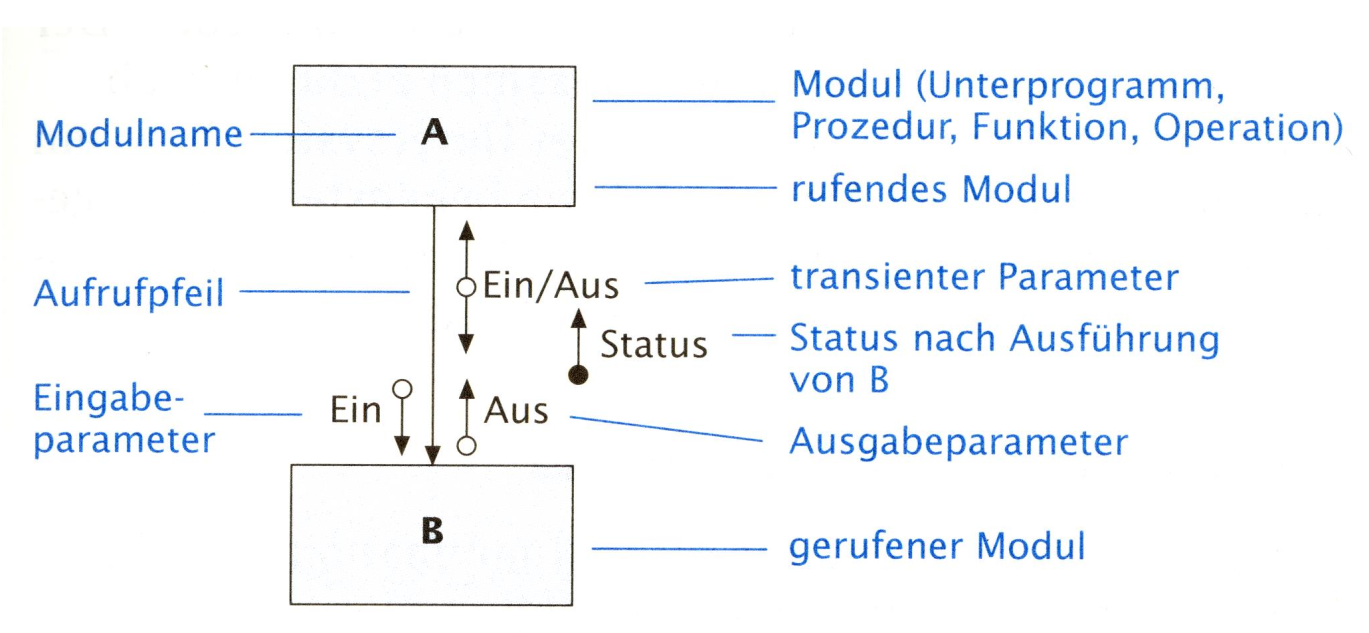
\includegraphics[width= \columnwidth]{images/structureChart.png}\\
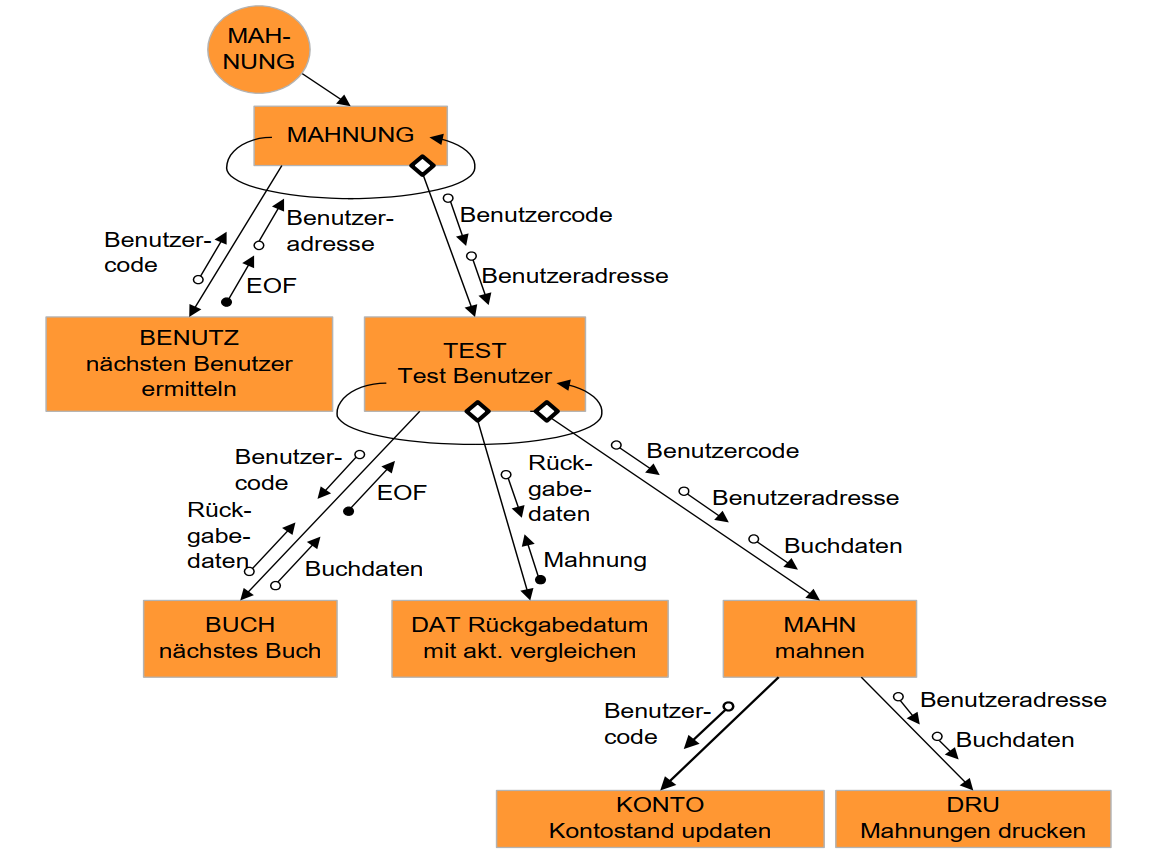
\includegraphics[width= \columnwidth]{images/bspStructChart.png}\\
\subsection{Nesting tree}
Indent tree \\
TODO Maybe add picture\\
\section{Datenbanken}
\subsection{Allgemein}
1. Vermeidung von Redundanz\\
2. Vermeidung von Insert-Anomalie\\
3. Vermeidung von Delete-Anomalie\\
4. Vermeidung von Update-Anomalie\\
\subsection{Normalformen}
\subsubsection{1. Normalform}
Jedem Datenfeld eines Datensatzes darf höchstens ein Wert
zugewiesen sein. D.h. es dürfen keine Mehrfacheinträge in einem Datenfeld vorliegen und Attribute müssen atomar sein.\\
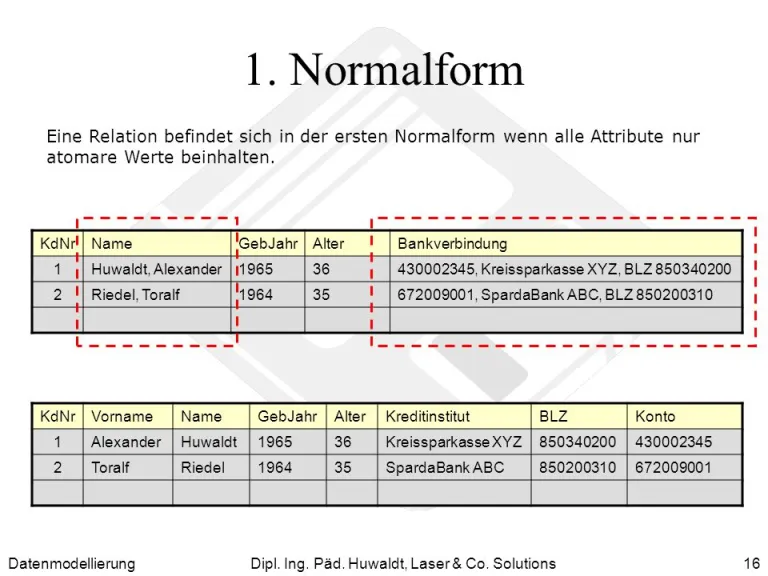
\includegraphics[width = 0.5\columnwidth]{images/1normalformEx.png}
\subsubsection{2. Normalform}
Erfüllt 1. Normalform \\
Eine Tabelle enthält nur Daten eines Themen- bzw. Informationsbereiches.\\
Aufteilung in mehrere Tabellen nach Themen/ Informationsgebieten.\\
Jedes Nicht-Schlüsselfeld  muss durch ein Schlüsselfeld identifizierbar sein und vom gesamten Schlüssel abhängen.\\
Überprüfen und ggf. neue Schlüsselfelder hinzufügen oder zusammengesetzte Schlüssel definieren.\\
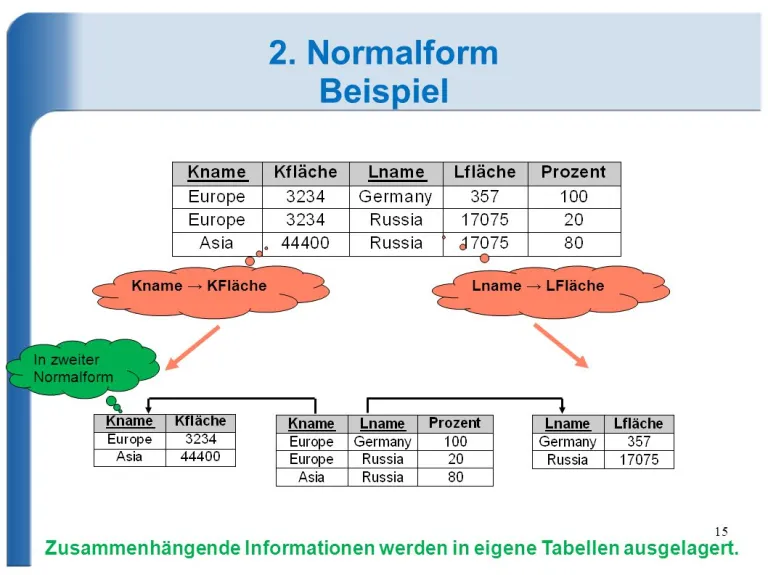
\includegraphics[width = 0.5\columnwidth]{images/2normalformEx.png}
\subsubsection{3. Normalform}
Aus keinem nicht Schlüsselattribut folgt ein anderes nicht Schlüsselattribut\\
Ist dann erfüllt, wenn die Tabelle die 2. Normalform erfüllt\\
Es dürfen keine transitiven (indirekten) Abhängigkeiten vorliegen.\\
Entfernung aller transitiven Abhängigkeiten durch Aufspalten der Tabelle in mehrere Tabellen, in denen alle Nicht-Schlüsselfelder direkt vom gesamten Schlüsselfeld abhängen\\
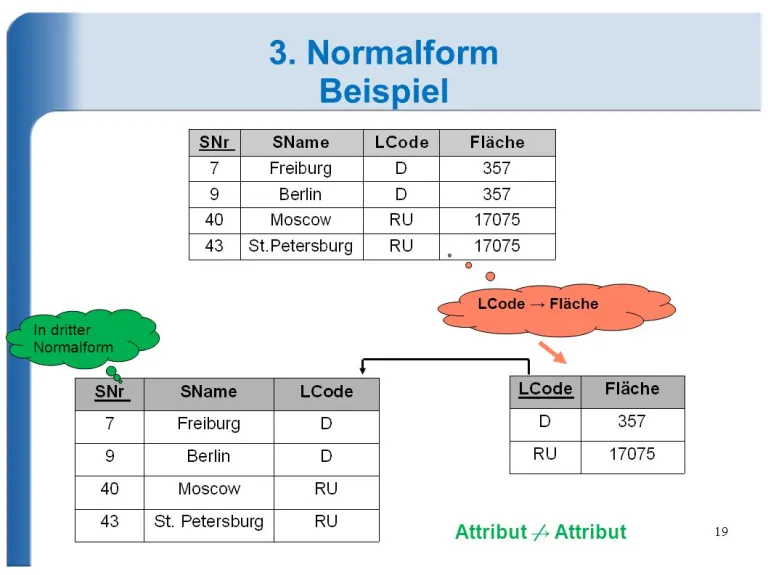
\includegraphics[width =0.5 \columnwidth]{images/3normalformEx.png}
\section{ERD}
\subsection{Kardinalitäten}
$\begin{array}{|c|c|c|c|c|}
    \hline & 1 & \text { C } & \text { M } & \text { CM } \\
    \hline 1 & (1: 1) & \text { (1:C) } & \text { (1:M) } & \text { (1:MC) } \\
    \hline \text { C } & (\mathrm{C}: 1) & \text { (C:C) } & \text { (C:M) } & \text { (C:MC) } \\
    \hline \mathrm{N} & (\mathrm{N}: 1) & \text { (N:C) } & \text { (N:M) } & \text { (N:MC) } \\
    \hline \mathrm{NC} & (\mathrm{NC}: 1) & \text { (NC:C) } & \text { (NC:M) } & \text { NC:MC } \\
    \hline
    \end{array}$
\begin{itemize}
    \item \textbf{1:} Genau 1
    \item \textbf{C:} 1 oder kein
    \item \textbf{M und N} mehrere
    \item \textbf{MC} kein, ein, oder mehrere
\end{itemize}
% \subsection{Example UML}
% 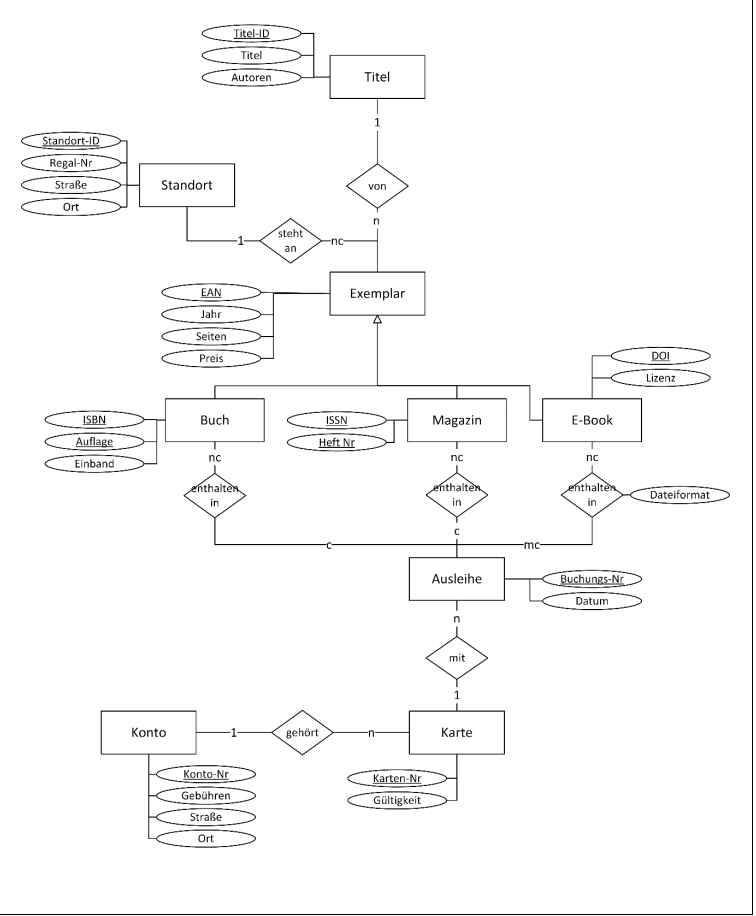
\includegraphics[width= \columnwidth]{images/erdbibbsp.png}
% \subsection{Crow's Notation}
% 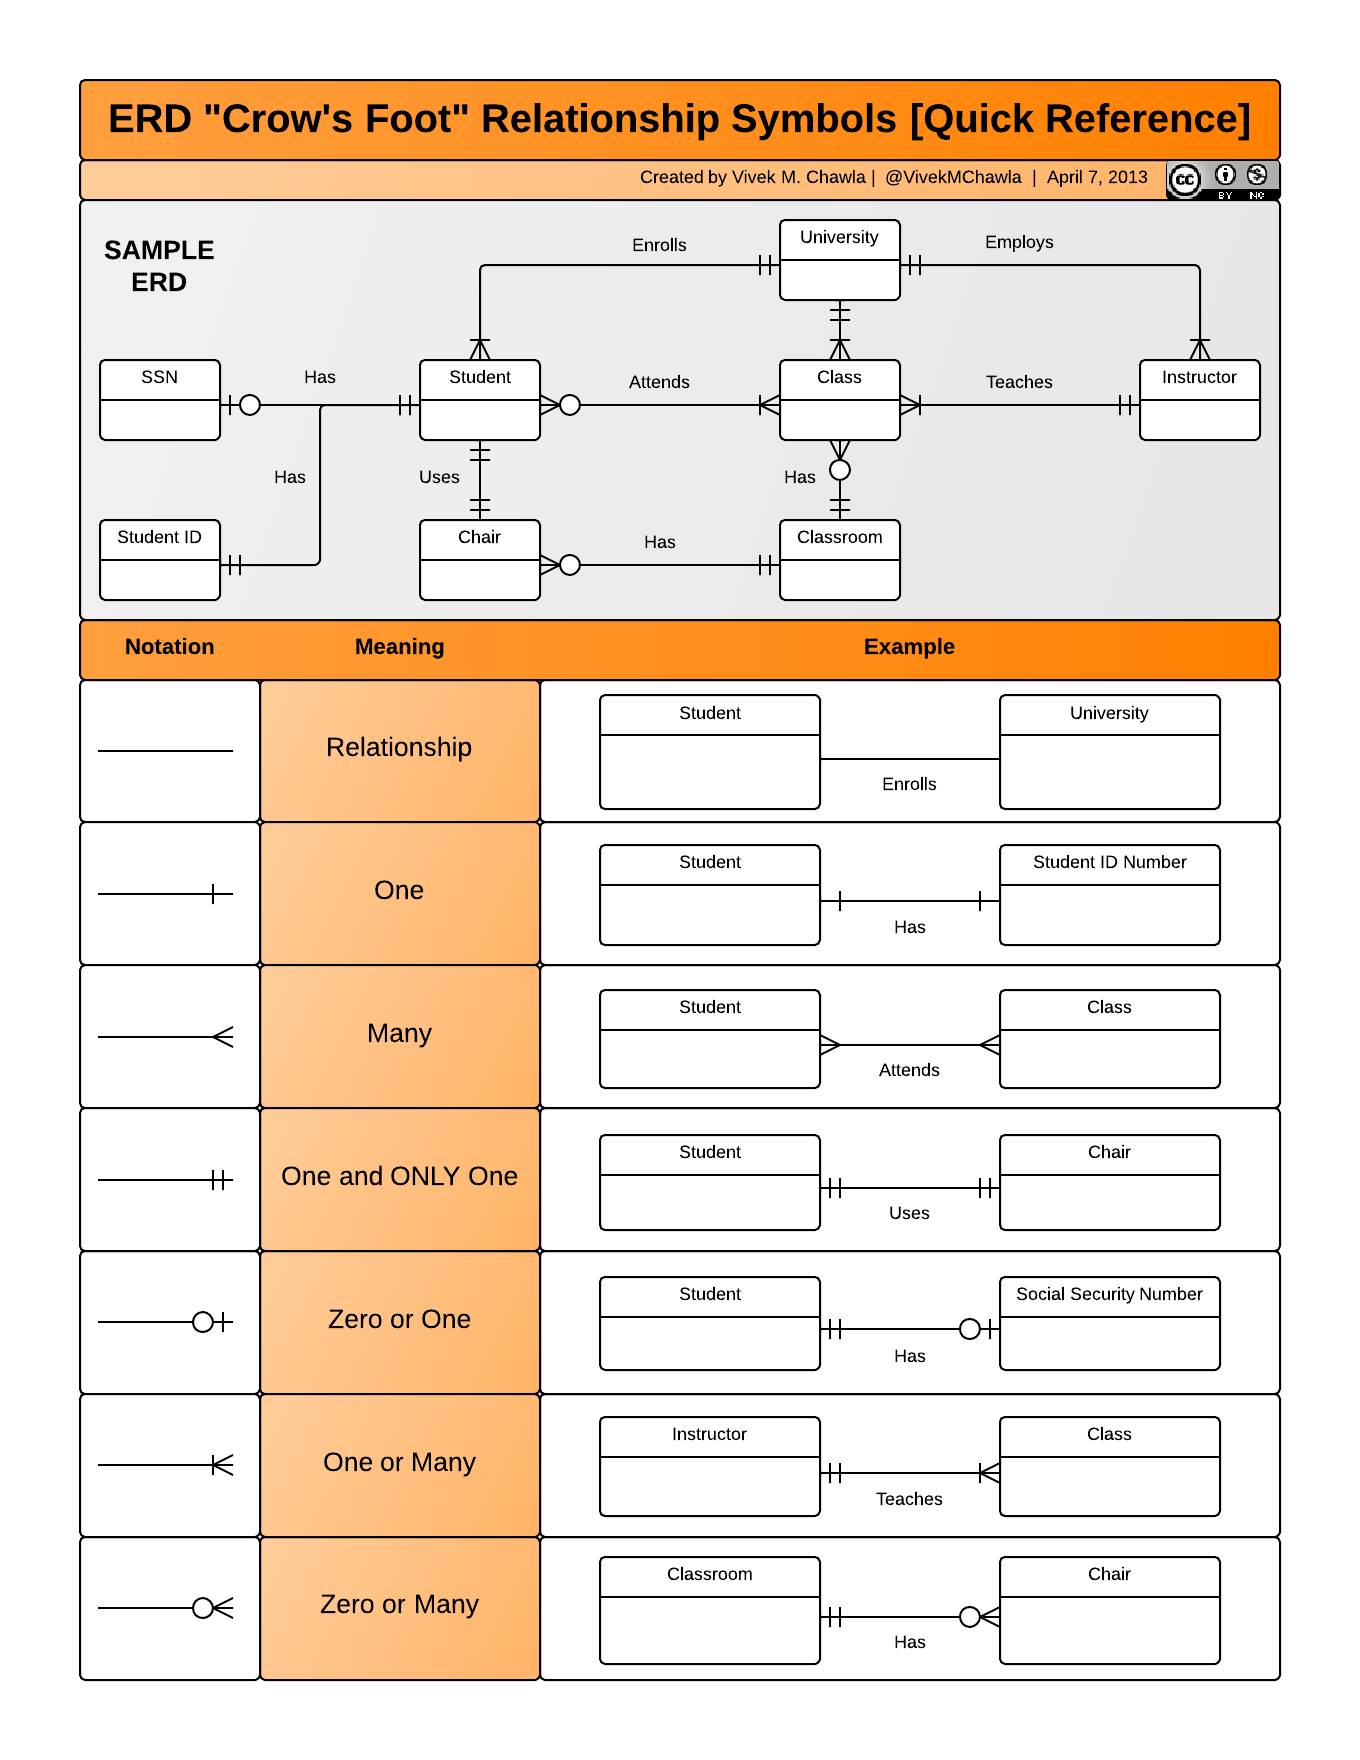
\includegraphics[width = \columnwidth]{images/5uwcF.png}\\
% 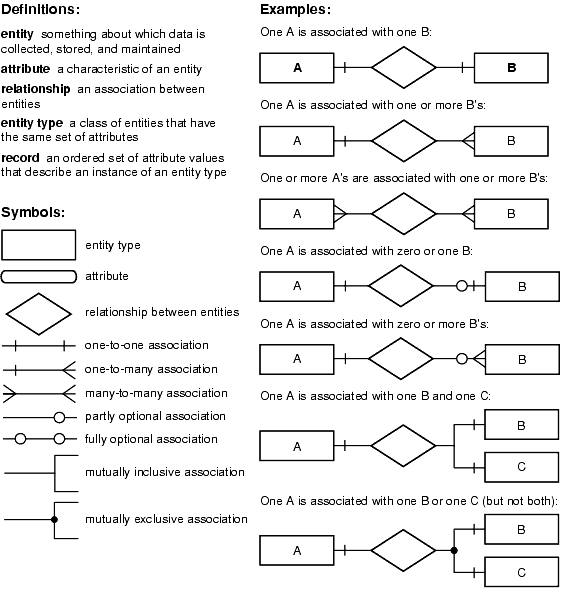
\includegraphics[width = \columnwidth]{images/9tvIZ.png}\\
\subsection{Implementierung}
\subsubsection{Vererbung}
Basis Entität bekommt foreign key ART-ID\\
Zusatztabelle: Basisentität ist ein mit primary key Art-ID und Attribut Art\\
Abgeleitete Entitäten bekommen Primary key der basis Entität als foreign key\\
\textbf{BSP}
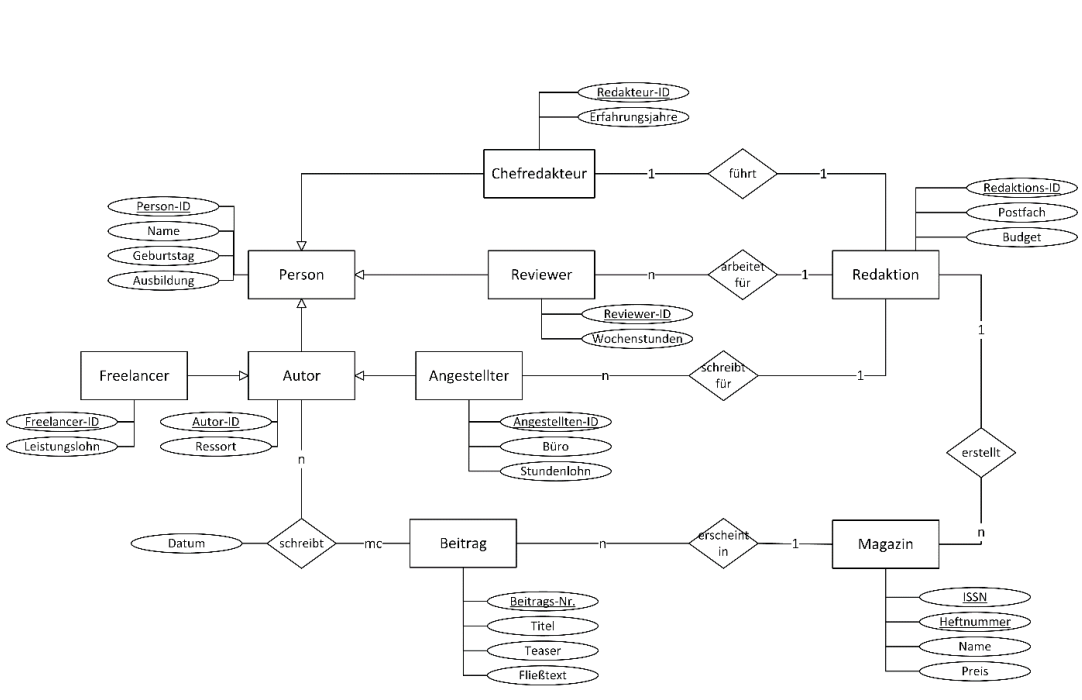
\includegraphics[width=0.78\columnwidth]{images/redaktionbsb.png}
\begin{tabular}{|l|}
    \hline
    \textbf{Person}\\
    \hline
    \underline{Person-ID}, Name, Birth, \dashuline{Person-Art-ID}\\
    \\
    \hline
\end{tabular}
\begin{tabular}{|l|}
    \hline
    \textbf{Person-ist-ein}\\
    \hline
    \underline{Person-Art-ID}, Art\\
    \\
    \hline
\end{tabular}
\begin{tabular}{|l|}
    \hline
    \textbf{Reviewer}\\
    \hline
    \underline{Reviewer-ID}, \dashuline{Person-ID}, Stunden, \dashuline{Redaktions-ID}\\
    \\
    \hline
\end{tabular}
\begin{tabular}{|l|}
    \hline
    \textbf{Chefredakteur}\\
    \hline
    \underline{Red-ID}, \dashuline{Person-ID}, Jahre, \dashuline{Redaktions-ID}\\
    \\
    \hline
\end{tabular}
\subsubsection{One-to-Many}
\textbf{One-Seite}\\
CREATE TABLE Autoren (
    \texttt{
    AutorID INT PRIMARY KEY,\\
    Name VARCHAR(255) NOT NULL,\\
    Geburtsdatum DATE
);}\\
\textbf{Many-Seite}\\
\texttt{CREATE TABLE Bücher (\\
    BuchID INT PRIMARY KEY,\\
    Titel VARCHAR(255) NOT NULL,\\
    Veröffentlichungsdatum DATE,\\
    AutorID INT,\\
    FOREIGN KEY (AutorID) REFERENCES Autoren (AutorID) ON DELETE SET NULL
);}
\subsubsection{Many-to-Many}
\texttt{
CREATE TABLE BuchAutoren (\\
    BuchID INT,\\
    AutorID INT,\\
    PRIMARY KEY (BuchID, AutorID),\\
    FOREIGN KEY (BuchID) REFERENCES Bücher (BuchID) ON DELETE CASCADE,\\
    FOREIGN KEY (AutorID) REFERENCES Autoren (AutorID) ON DELETE CASCADE
);}
\subsubsection{Anzahl auftreten aus Relation}
\textbf{BSP: Autorenanzahl pro Buch}\\
\texttt{
SELECT b.BuchID, b.Titel, COUNT(ba.AutorID) AS AnzahlAutoren\\
FROM Bücher b\\
LEFT JOIN BuchAutoren ba ON b.BuchID = ba.BuchID\\
GROUP BY b.BuchID, b.Titel\\
ORDER BY b.BuchID;\\
}
% \columnbreak
\section{SQL}
\subsection{Befehle}
\textbf{DISTINCT:} Gibt nur eindeutige Werte ohne Duplikate
\subsection{Select from n based on limit in n}
Alle Tests aus den 5 Laboren mit dem höchsten Budget\\
\texttt{
    SELECT Test.ID, Test.Datum, Labor.Name\\
    FROM Test\\
    INNER JOIN Labor ON Test.LaborID = Labor.LaborID\\
    WHERE Test.Risiko > 2\\
    AND Labor.LaborID IN (\\
        SELECT LaborID\\
        FROM Labor\\
        ORDER BY Budget DESC\\
        LIMIT 5\\
    );\\
}
\textbf{BSB: Create table from ERD}
\texttt{
    CREATE TABLE Spielmaterial (
Material-Nr INT NOT NULL,\\
Art VARCHAR(50) NOT NULL,\\
Farbe VARCHAR(15) NOT NULL,\\
Beschriftung VARCHAR(50) NOT NULL,\\
Gewicht DOUBLE NOT NULL,\\
Spiel-ID INT NOT NULL,\\
PRIMARY KEY (Material-Nr),\\
FOREIGN KEY (Spiel-ID) REFERENCES Spiel(Spiel-ID));\\
}
\section{GAIA}
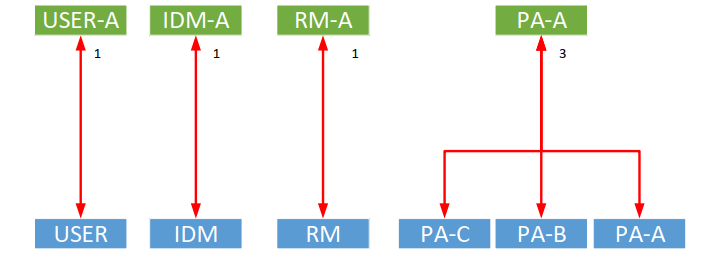
\includegraphics[width=\columnwidth]{images/agentenmodell.png}
\subsection{Role Model Template}
\begin{tabular}{|l|l|}
    \hline
    Role Schema:&\\
    \hline
    Description:&\\
    \hline
    Protocols and \underline{Activities}: & \\
    \hline
    Permissions:  & - reads:\\
    & - changes:\\
    & - generates:\\
    \hline
    Responsibilities: & - Liveness:\\
    & - Safety:\\
    \hline
\end{tabular}\\
\begin{itemize}
    \item Protokolle und Aktivitäten (Protocols and Activities)
    \begin{itemize}
        \item Protokolle legen fest, wie verschiedene Rollen miteinander interagieren;
        \item Aktivitäten sind Aufgaben, die von einer Rolle ohne Interaktion erledigt werden.
    \end{itemize}
    \item Rechte (Permissions)
    \begin{itemize}
        \item Hier werden die Rechte zum Lesen, Ändern und Erzeugen von Datenelementen spezifiziert.
    \end{itemize}
    \item Verantwortlichkeiten (Responsibilities)
    \begin{itemize}
        \item Verantwortlichkeiten werden in zwei Kategorien unterteilt: Lebendigkeit (Liveness) und Sicherheit (Safety).
        \begin{itemize}
            \item Liveness beschreibt die Reihenfolge der Aufgaben, die von der Rolle realisiert werden müssen. Sie setzen sich aus den im ersten Bereich beschriebenen Protokollen und Aktivitäten
            zusammen.
            \item Safety sind Bedingungen (Invarianten), die eingehalten werden müssen, um unerwünschte
            oder sogar gefährliche Situationen zu vermeiden.
        \end{itemize}
    \end{itemize}
\end{itemize}
\subsection{BSB Role Description}
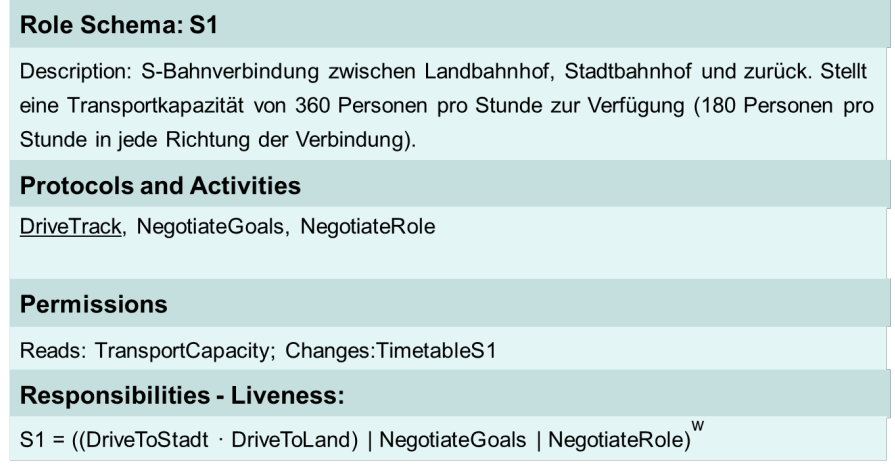
\includegraphics[width=\columnwidth]{images/gaiarolesbsp.png}
\subsection{Template for Interaction Model}
\begin{tabular}{|c|c|}
    \hline
    [Protocol's name]  &[Inputs]\\
    \hline
    [Initiator] \quad \vline  \quad [Responder] & \\
    \hline
    [Description] & [Outputs] \\
    \hline
\end{tabular}
\begin{itemize}
    \item Description: Beschreibung
    \item Initiator: Rolle
    \item Responder: Rolle
    \item Inputs: Informationen des Auslösers
    \item Outputs: Informationen des Beantworters
\end{itemize}
\subsection{Operatoren Ablaufbeschreibung}
\begin{tabular}{ll}
    Operator & Interpretation\\
    $x . y$ & x followed by y\\
    $x|y  $ & x or y occurs\\
    $x^* $ & x occurs 0 or more times\\
    $X+$  & x occurs 1 or more times\\
    $x^{\omega}$ & x occurs innately often\\
    $\left[x\right]$ & x is optional\\
    $ x || y $ & x and y are interleaved(verschachtelt)
\end{tabular}
\subsection{Service Model}
\begin{tabular}{|c|c|c|c|c|}
    \hline
    Service & Inputs & Outputs & Precondition& Post-condition \\
    \hline
    &&&&\\
    \hline    
\end{tabular}
%  Nesting tree and Structure chart, empty circle is data flow full circle is control flow folien ue5
% TODO ER Diagramme cheat sheet
% TODO Revisit ex8 last task
\section{SQL Beispiele}
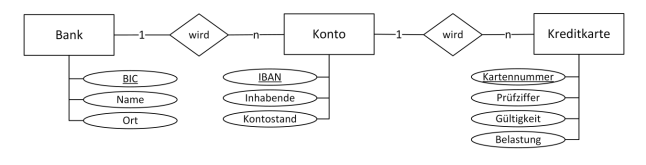
\includegraphics[width= \columnwidth]{images/ss21erd.png}\\
\rule{\columnwidth}{0.5pt}
    Erstellen Sie eine SQL-Anweisung, welche die Tabelle Konto mit ihren zugehörigen
    Attributen der Datenbank hinzufügt.:\\
    \rule{\columnwidth}{0.5pt}
    CREATE TABLE Konto (\\
        IBAN Varchar(22) NOT NULL,\\
        Inhabende Varchar(50) NOT NULL,\\
        Kontostand INT,\\
        BIC Varchar(11) NOT NULL,\\
        PRIMARY KEY (IBAN),\\
        FOREIGN KEY (BIC) REFERENCES Bank(BIC));\\
        \rule{\columnwidth}{0.5pt}
        Erstellen Sie eine SQL-Anweisung, welche die Kontodaten (IBAN, BIC, Bankname
        und Inhabende) aller Konten von Stuttgarter Banken aufsteigend sortiert nach
        "Inhabende" ausgibt.:\\
        \rule{\columnwidth}{0.5pt}
        SELECT Bank.Name, Bank.BIC, Konto.IBAN, Konto.Inhabende\\
        FROM Konto\\
        JOIN Bank USING (BIC)\\
        WHERE Bank.Ort = “Stuttgart”\\
        ORDER BY Konto.Inhabende ASC;
        \rule{\columnwidth}{0.5pt}
        Erstellen Sie eine SQL-Anweisung, welche die IBAN und das gesparte Geld gruppiert
nach Konten mit weniger als 10.000€ und aufsteigend sortiert nach dem gesparten
Geld auflistet. Dabei berechnet sich das gesparte Geld als Differenz des Kontostandes
und der Summe aller Kreditkartenbelastungen. Es sollen nur die ersten 100 Treffer
ausgegeben werden.
\rule{\columnwidth}{0.5pt}
SELECT Konto.IBAN,\\
Konto.Kontostand-SUM(Kreditkarte.Belastung) AS Geld\\
FROM Konto LEFT JOIN Kreditkarte USING(IBAN)\\
GROUP BY Konto.IBAN HAVING Geld < 10000\\
ORDER BY Geld\\
LIMIT 100;
\rule{\columnwidth}{0.5pt}
Erstellen Sie eine SQL-Anweisung, welche den 100 ärmsten Konten der Konten in
Stuttgart die einen Kontostand unter 10.000 € aufweisen 5.000€ gutschreibt.
\rule{\columnwidth}{0.5pt}
UPDATE Konto\\
LEFT JOIN Bank USING(BIC)\\
SET Konto.Kontostand = Konto.Kontostand + 5000\\
WHERE Konto.Kontostand < 10000 AND Bank.Ort = “Stuttgart“\\
ORDER BY Konto.Kontostand\\
LIMIT 100;\\
\rule{\columnwidth}{0.5pt}
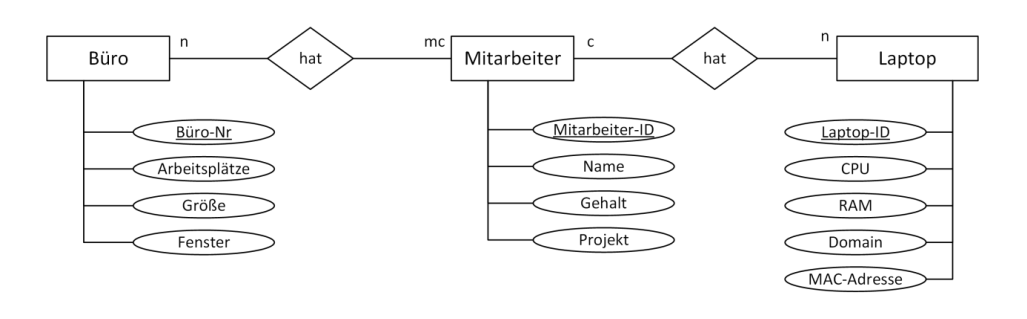
\includegraphics[width= \columnwidth]{images/ws20erd.png}\\
\rule{\columnwidth}{0.5pt}
Erstellen Sie eine SQL-Anweisung, welche die Tabelle Laptop mit ihren zugehörigen
Attributen der Datenbank hinzufügt.
\rule{\columnwidth}{0.5pt}
CREATE TABLE Laptop (\\
Laptop-ID INT NOT NULL,\\
CPU DOUBLE NOT NULL,\\
RAM INT NOT NULL,\\
Domain Varchar(30) NOT NULL,\\
MAC-Adresse Varchar(17) INT NOT NULL,\\
Mitarbeiter-ID INT NOT NULL,\\
PRIMARY KEY (Laptop-ID),\\
FOREIGN KEY (Mitarbeiter-ID) REFERENCES\\
Mitarbeiter(Mitarbeiter-ID));\\
\rule{\columnwidth}{0.5pt}
Erstellen Sie eine SQL-Anweisung, die ermittelt wie viele Laptops mit 4GB RAM
oder weniger in den einzelnen Projekten existieren.
\rule{\columnwidth}{0.5pt}
SELECT COUNT(Laptop-ID), Mitarbeiter.Projekt FROM Laptop\\
INNER JOIN Mitarbeiter ON Mitarbeiter.Mitarbeiter-ID =\\
Laptop.Mitarbeiter-ID\\
WHERE Laptop.RAM <= 4GB\\
GROUP BY Mitarbeiter.Projekt;\\
\rule{\columnwidth}{0.5pt}
Erstellen Sie eine SQL-Anweisung, welche die Anzahl der Mitarbeiter pro Büro
unterteilt in die Projekte auflistet. Die Büro-Nr. sollen absteigend und die Projekte
aufsteigend sortiert sein.
\rule{\columnwidth}{0.5pt}
SELECT COUNT(Mitarbeiter.Mitarbeiter-ID),\\
Mitarbeiter.Projekt, Büro.Büro-Nr FROM Büro\\
LEFT JOIN Büro-Mitarbeiter-Rel rel ON rel.Büro-Nr =\\
Büro.Büro-Nr\\
LEFT JOIN Mitarbeiter ON Mitarbeiter.Mitarbeiter-ID =\\
rel.Mitarbeiter-ID\\
GROUP BY Büro.Büro-Nr, Mitarbeiter.Projekt\\
ORDER BY Büro.Büro-Nr ASC, Mitarbeiter.Projekt DESC;\\
\rule{\columnwidth}{0.5pt}
Erstellen Sie eine SQL-Anweisung, welche die Laptops mit 4GB RAM oder weniger
auf 8GB aufrüstet, wenn der zugeordnete Mitarbeiter ein Gehalt über 30.000 hat.
\rule{\columnwidth}{0.5pt}
UPDATE Laptop\\
INNER JOIN Mitarbeiter ON Laptop.Mitarbeiter-Nr =\\
Mitarbeiter.Mitarbeiter-Nr\\
SET Laptop.RAM=8\\
WHERE (Laptop.RAM <= 4 AND Mitarbeiter.Gehalt > 30000)\\
\rule{\columnwidth}{0.5pt}
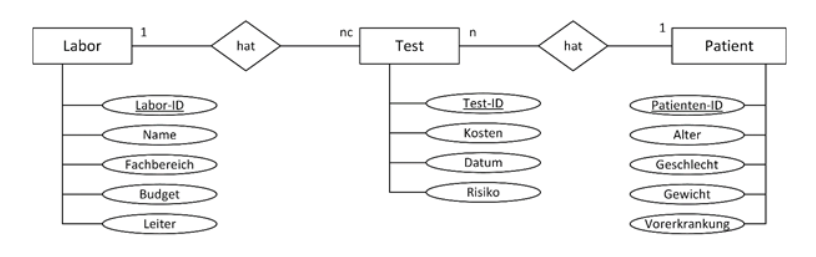
\includegraphics[width= \columnwidth]{images/ss20erd.png}\\
\rule{\columnwidth}{0.5pt}
Erstellen Sie eine SQL-Anweisung, welche die Tabelle Test mit ihren zugehörigen
Attributen der Datenbank hinzufügt.
\rule{\columnwidth}{0.5pt}
CREATE TABLE Test (\\
Test-ID INT NOT NULL,\\
Kosten DOUBLE NOT NULL,\\
Datum DATE NOT NULL,\\
Risiko INT NOT NULL,\\
Labor-ID INT NOT NULL,\\
Patienten-ID INT NOT NULL,\\
PRIMARY KEY (Test-ID),\\
FOREIGN KEY (Labor-ID) REFERENCES Labor(Labor-ID),\\
FOREIGN KEY (Patienten-ID) REFERENCES Patient(Patienten-ID));\\
\rule{\columnwidth}{0.5pt}
Erstellen Sie eine SQL-Anweisung, welche die Gesamtkosten aller Tests der Patienten mit
einem Alter unter 50 ermittelt, die in den Monaten Januar bis Juni 2020 durchgeführt
wurden.
\rule{\columnwidth}{0.5pt}
SELECT SUM(Kosten) FROM Test\\
JOIN Patient ON Patient.Patienten-ID = Test.Patienten-ID\\
WHERE Patient.Alter < 50 AND\\
Test.Datum BETWEEN 2020-01-01 AND 2020-06-30;\\
\rule{\columnwidth}{0.5pt}
Erstellen Sie eine SQL-Anweisung, welche alle Test-IDs, das Testdatum und den
zugehörigen Labornamen der fünf Labore mit dem größten Budget ausgibt. Dabei sollten
nur Ergebnisse gelistet werden, die Tests mit einer Risikostufe größer 2 betreffen.
\rule{\columnwidth}{0.5pt}
SELECT Test.ID, Test.Datum, Labor.Name FROM Test\\
INNER JOIN (\\
SELECT DISTINCT Labor.Name FROM Labor\\
ORDER BY Labor.Budget DESC\\
LIMIT 5\\
) AS Laborliste ON Laborliste.Labor-ID = Test.Labor-ID\\
INNER JOIN Labor ON Labor.Labor-ID=Laborliste.Labor-ID\\
WHERE Test.Risiko > 2;\\
\rule{\columnwidth}{0.5pt}
Erstellen Sie eine SQL-Anweisung, welche die ältesten 10.000 Testergebnisse löscht, die
ein Risiko kleiner gleich 2 besitzen und vor Januar 2020 erstellt wurden oder vor dem Jahr
2016 erstellt wurden.
\rule{\columnwidth}{0.5pt}
DELETE FROM Test
WHERE Test.Risiko < 3 AND Test.Datum < 2020-01-01\\
OR Test.Datum < 2016-01-01\\
ORDER BY Test.Datum ASC\\
LIMIT 10000;
\section{CTL-Beispiele}
\begin{tabular}{|p{0.45 \columnwidth}|p{0.45 \columnwidth}|}
    \hline
    $\text { !S0|!S3|!S7 } \rightarrow \text { EX S7 }$ & Es soll außer von S0, S3 und S7 immer der "Chat mit dem Servicemitarbeiter" direkt
    gestartet werden können\\
    \hline
    $\text { EX S4 }$ & Da Daten zum Einloggen auch gespeichert werden können, soll es optional möglich
    sein, nach dem Start des Webservice direkt in den Zustand Einloggen (S4) zu
    gelangen.\\
    \hline
    $\mathrm{S} 7 \rightarrow \mathrm{AX} \mathrm{S} 1$ & Da Daten zum Einloggen auch gespeichert werden können, soll es optional möglich
    sein, nach dem Start des Webservice direkt in den Zustand Einloggen (S4) zu
    gelangen.\\
    \hline
    $\text { AG EF S3 }$ & Am Ende wird der Webservice immer geschlossen.\\
    \hline
    $\text { EG EX a }$  & Auf mindestens einem Pfad folg in jedem Zustand, dass entlang mindestens einem Pfad in
    im unmittelbar nächsten Zustand a gilt.\\
    \hline
    $\mathbf{A G}(\mathrm{b} \rightarrow \mathbf{A X}(\mathrm{n} \mid \mathrm{m}))$ &Auf allen Pfaden gilt in jedem Zustand, wenn b gilt dann gilt auf allen Pfaden im unmittelbar nachfolgenden Zustand $\mathrm{n}$ oder $\mathrm{m}$.\\
    \hline
    $\text { AG }(\mathrm{c} \rightarrow \mathrm{EF} !(\mathrm{c} \& \mathrm{u}))$  &Entlang aller Pfade in allen Zuständen gilt: wenn c gilt, dann gilt auf mindestens einem Pfad irgendwann auch in einem Zustand c und u nicht zusammen.\\
    \hline
    $\mathbf{A G}(\mathrm{d} \mathbf{U} \mathrm{v}) \mid \mathbf{A X} \mathrm{y}$&
    Entlang aller Pfade in allen Zuständen gilt: Auf allen Pfaden gilt d bis zum Erreichen von y oder auf allen Pfaden folgt unmittelbar ein Zustand in dem y gilt.\\
    \hline
    $\text { AG ,,Wasserst. überw.“ }$ & In allen Zuständen wird "Wasserstand überwachen" durchgeführt.\\
    \hline
    $\mathrm{AG}(\mathrm{S} 2|\mathrm{~S} 3| \mathrm{S} 4) \rightarrow \text { EX S5 }$ & Sobald Wasser in der Maschine ist muss es immer möglich sein in den "Wasser
    abpumpen" Zustand zu wechseln.\\
    \hline
    $\mathrm{AG}(\mathrm{S} 5 \rightarrow \mathrm{AX} \mathrm{S} 1)$ &Wasser abpumpen wird erst beendet, wenn kein Wasser mehr in der Maschine ist\\
    \hline
    $\text { AG(!S6 U S1) }$&Nur wenn kein Wasser mehr in der Waschmaschine ist, kann der Waschvorgang
    abgeschlossen werden.\\
    \hline
    $\text { AG AX } \mathrm{a}$  & Auf allen Pfaden in jedem Zustand gilt, dass entlang aller Pfaden in jedem nächsten Zustand a gilt (= a gilt immer! solche Formulierung nur halber Punkt!).\\
    \hline
    $\mathbf{E G}(\mathrm{b} \rightarrow \mathbf{A X}(\mathrm{r} \mid \mathrm{s}) \boldsymbol{\&} \mathbf{A X}(\mathrm{s} \rightarrow \mathrm{q}))$ & Auf mindestens einem Pfad gilt in jedem Zustand, wenn b gilt dann gilt auf allen Pfaden im unmittelbar nachfolgenden Zustand $\mathrm{r}$ oder $\mathrm{s}$ und wenn s gilt dann gilt auch $\mathrm{q}$.\\
    \hline
    $\mathbf{E G}(\mathrm{c} \rightarrow \mathbf{A F}(\mathrm{c} \& \mathrm{z}))$ & Es existiert mindestens ein Pfad auf dem, wenn c gilt dann gilt, auf allen Pfaden irgendwann auch $\mathrm{c}$ und $\mathrm{z}$ zusammen.\\
    \hline
    $\text { :x } \rightarrow \mathrm{A}(\mathrm{d} \mathbf{W} \mathrm{y}) \mid \mathbf{E X} \mathrm{y}$ & Wenn nicht $\mathrm{x}$ gilt dann gilt $\mathrm{d}$ immer oder bis zum Erreichen von $\mathrm{y}$ oder auf mindestens einem Pfad folgt unmittelbar $\mathrm{y}$.\\
    \hline
    $\mathbf{E X}(! \mathrm{e} \rightarrow \mathbf{A}(\mathrm{v} \mathbf{U} \mathrm{w}))$ & Entlang mindestens einem Pfad folgt unmittelbar dass wenn nicht e gilt, dann gilt immer $\mathrm{v}$ bis zum ersten Auftreten von w und w muss auftreten\\
    \hline
\end{tabular}
\end{multicols*}
\end{document}